\documentclass[conference]{IEEEtran}
\IEEEoverridecommandlockouts
% The preceding line is only needed to identify funding in the first footnote. If that is unneeded, please comment it out.
\usepackage{cite}
\usepackage{amsmath,amssymb,amsfonts}
\usepackage{algorithmic}
\usepackage{graphicx}
\usepackage{textcomp}
\usepackage{xcolor}
\usepackage[binary-units=true]{siunitx}
\usepackage{subcaption}
\usepackage{booktabs}
\usepackage{hyperref}
\def\BibTeX{{\rm B\kern-.05em{\sc i\kern-.025em b}\kern-.08em
    T\kern-.1667em\lower.7ex\hbox{E}\kern-.125emX}}
\begin{document}

\title{Learning Robot Poses from Artificial Images\\
%{\footnotesize \textsuperscript{*}Note: Sub-titles are not captured in Xplore and
%should not be used}
}

\newif\iffinalcopy

% comment this lind to make paper valid for blind review
%\finalcopytrue

\iffinalcopy

    \author{
        \IEEEauthorblockN{
            Christoph Heindl\IEEEauthorrefmark{1}, 
            Sebastian Zambal\IEEEauthorrefmark{1}, 
            Markus Ikeda\IEEEauthorrefmark{1}, 
            Andreas Pichler\IEEEauthorrefmark{1}, and 
            Josef Scharinger\IEEEauthorrefmark{2}
        }
        \\
        \IEEEauthorblockA{
            \IEEEauthorrefmark{1}\textit{PROFACTOR GmbH} \\ 4407 Steyr, Austria\\ \texttt{firstname.lastname@profactor.at}
        }
        \\
        \IEEEauthorblockA{
            \IEEEauthorrefmark{2}\textit{Institute of Computational Perception} \\ Johannes Kepler University \\ 4040 Linz, Austria\\ \texttt{josef.scharinger@jku.at}
        }
    }

\else

    \author{
        \IEEEauthorblockN{
            Author
        }
        \\
        \IEEEauthorblockA{
            \IEEEauthorrefmark{1}\textit{Affiliation}
        }
    }

\fi


\maketitle

\begin{abstract}
    Impressive results have been achieved in computer vision via deep learning methods over the last years. However, the lack of supervised data has led to a slowdown in the progress of deep learning in many specialized areas. This work considers the task of robot pose estimation in color images using artificial training data. We propose a highly parallel data generation workflow, in which the simulator engine is directly looped into the training procedure. A feedback mechanism enables more effective model learning, by focusing the simulator on highly valuable samples for training. We demonstrate that our model, trained on artificial robot images, is able to generalize to real world images. 
\end{abstract}

\begin{IEEEkeywords}
machine learning, artificial data, data augmentation
\end{IEEEkeywords}

\section{Introduction and Related Work}
The remarkable results of supervised deep learning in the field of robotics and computer vision are to a large extent due to the availability of annotated data sets. Up until recently most of the annotation was carried out by domain experts. This time consuming process significantly slows down the progress of deep learning efforts. In many tasks it is difficult, in most niche areas impossible, to obtain strong supervision because of the high costs.

Exposed to this bottleneck, new fields of research have opened up. Active learning \cite{druck2009active, settles2012active, cakmak2012designing} attempts to use human experts in a more targeted way by focusing on samples that seem to be of highest value for learning task. Semi-supervised learning \cite{chapelle2009semi, salimans2016improved, zhu2006semi} combines large unlabeled data sets with smaller labeled data sets through structural assumptions, such as smoothness or low-dimensionality constraints. Transfer learning \cite{pratt1993discriminability, ventura2007theoretical, pan2010survey} exploits the fact that models trained on specific tasks can be adapted to related problems using fewer training samples. Weak supervision \cite{ratner2016data, zhou2017brief} is motivated by leveraging less precise, higher level supervision that is often easier to obtain. This includes heuristics, weak or biased classifiers, unreliable non-experts. 

\begin{figure}[htbp]
    \centerline{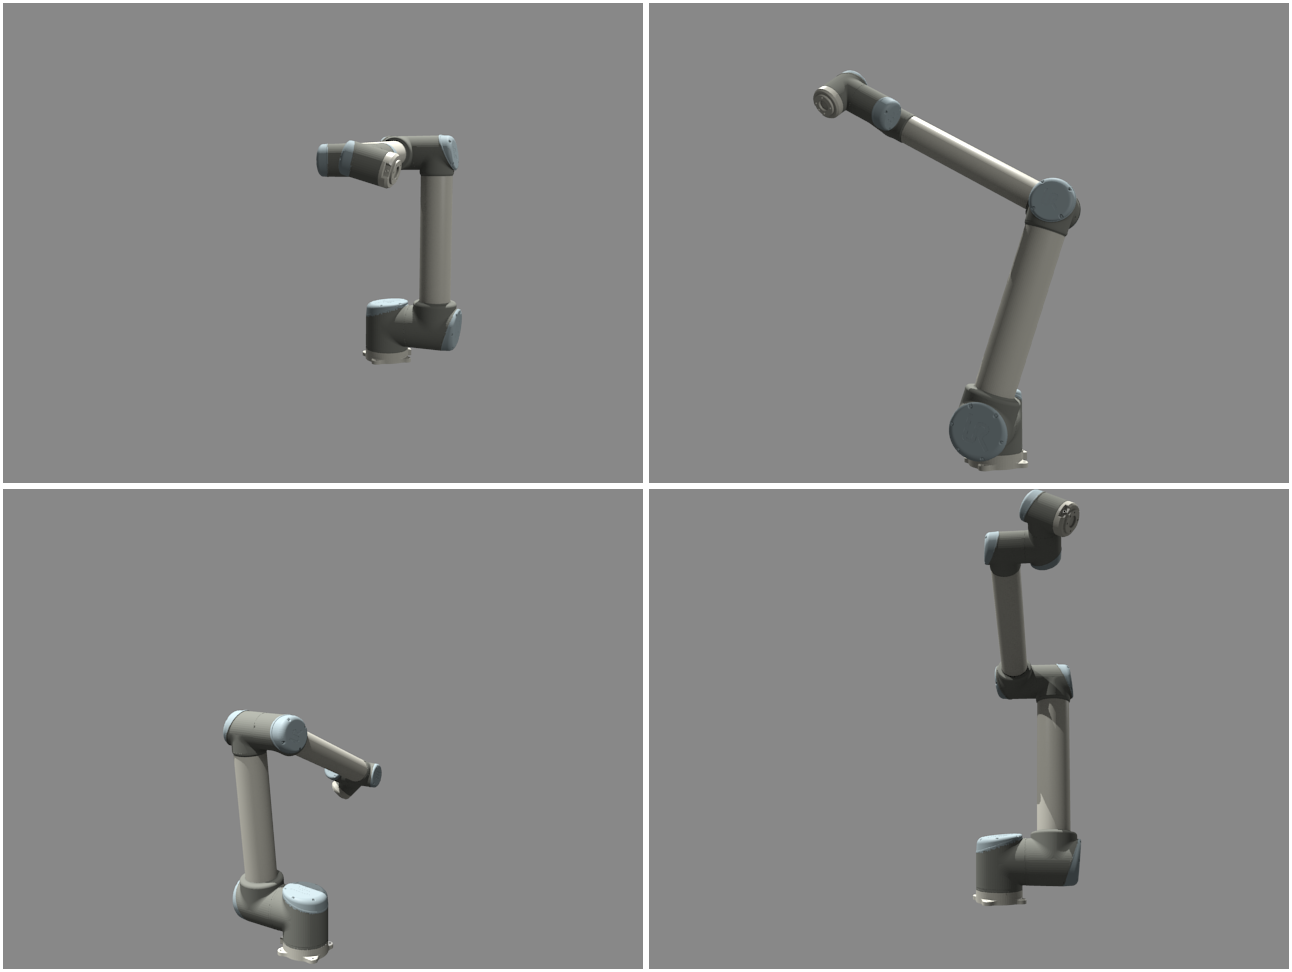
\includegraphics[width=0.9\columnwidth]{figures/examplesUR10/renderedImages.png}}
    \caption{\label{fig:ur10examples} Examples of training images with UR10 robots rendered in Blender (left) and with random background images added (right).}
\end{figure}

% https://hazyresearch.github.io/snorkel/blog/ws_blog_post.html

In contrast to the methods mentioned above, synthetic data generation drops the necessity for real world annotated data in favor of artificial data sources. Synthesized data is available in virtually infinite variety and is de-facto auto-labelled. This has led to variety of successful applications in different domains: Jaderberg et al. \cite{jaderberg2014synthetic} have demonstrated natural scene text recognition from synthetic data, Peng et al. \cite{peng2015learning} trained object detectors from 3D models and Johnson et al. \cite{2017_Johnson_DrivingInTheMatrix} used photo-realistic computer rendering captured from a game engine to train car detectors. A common theme to all of these synthetic approaches is the following: (a) a simulator engine generates artificial training data, (b) the generated data is stored to disk and (c) the offline data stack is used for training. The main shortcomings to this approach are early training data commitment and the lack of adaptability of data generation to training demands.

Considering pose estimation from images, the majority of the machine learning approaches are based on real-world hand-annotated data sets. Nowadays comprehensive datasets for human pose estimation, such as COCO \cite{lin2014microsoft} and MPII Multi-Person Dataset \cite{andriluka20142d}, exist. Pictorial methods \cite{fischler1973representation, felzenszwalb2005pictorial} represent individual parts of the body arranged in a deformable network. With the success of deep learning, convolutional networks \cite{oliveira2016deep} predicting all body part locations superseded individually trained detectors. In multi pose detection two approaches have become established: in the top-down approach \cite{gkioxari2014using, sun2011articulated} an upstream detector singles out individual instances. The bottom-up approach identifies instance independent features, such as joint locations, and fusions them into body instances \cite{insafutdinov2016deepercut, wei2016convolutional}. Our network is based on the work of Heindl et al. \cite{cheind2019disp} which builds upon work done by Cao et al. \cite{cao2017realtime}.

In contrast to human pose datasets, image based databases for robot pose detection are not standardized for various reasons: (a) robots are expensive in acquisition, (b) the required infrastructure and personal for operating them is complex and (c) accurate annotation through crowdsourcing is more difficult to obtain. The research has therefore focused on training based on smaller hand-labelled datasets \cite{miseikis2018multi, miseikis2018transfer, garcia2013guidance, varhegyivisual}, or highly specialized data sets \cite{levine2018learning}.

In this paper we propose to train solely on non-photorealistic artificial generated image data (figure \ref{fig:ur10examples}). Such data is much simpler to produce. We propose a learning framework composed of a simulator engine that is directly looped into mini-batch learning. This allows us to avoid early data commitment. Additionally, a bi-directional communication channel enables the simulation to adapt sampling towards training needs. We demonstrate the usefulness of our approach in detection of robot poses.


\section{Method}

    Our approach is outlined in Figure \ref{fig:architecture}. Without loss of generality we consider a supervised regression task. One or more simulator engines generate independent and identically distributed training tuples $\{(\textbf{x},\textbf{y},\textbf{h})\} \sim \mathrm{P}(\textbf{X},\textbf{Y},\textbf{H};\theta)$ by sampling from a probabilistic graphical model parametrized by $\theta$. The training samples $\{(\textbf{x},\textbf{y})\}$ are used for mini-batch updating the parameters $\phi$ of a neural network $\mathrm{P}(\textbf{Y} \lvert \textbf{X};\phi)$. Finally, the simulation parameters $\theta$ are adapted via a feedback signal emitted from a control unit.

    \begin{figure}[htbp]
        \centerline{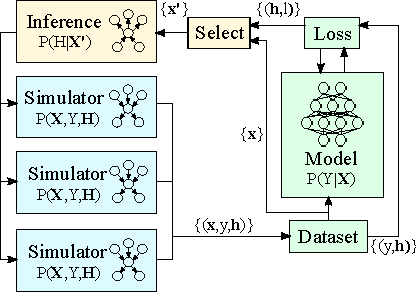
\includegraphics[width=0.9\columnwidth]{figures/architecture/overview.pdf}}
        \caption{\label{fig:architecture} Architecture of our system.}
    \end{figure}
    
    In the following we outline individual elements of our system. In section \ref{sec:artificialData} we describe the simulator. In section \ref{sec:model} we outline details about the neural network model. We explain the control block for feedback in section \ref{sec:feedback} and finally provide implementation details in section \ref{sec:impl}.


\subsection{Artificial Data for Training}
    \label{sec:artificialData}

    Conceptually, the process of creating randomized artificial training data can be expressed in terms of a  probabilistic graphical model. Such a model describes probabilistic between hidden and observed variables in terms of prior and conditional probability distributions. The observed variables in our model correspond to pixels of generated images $\mathbf{X}$. The hidden variables describe the model behind these images. Hidden variables $\mathbf{H}$ consist of robot joint angles and virtual camera position. To be more specific, we can write the hidden parameters of the model as a vector of random variables $\mathbf{H} = (J_1, \dots, J_6, R, \Delta, \Gamma, D, B)$. $J_i$ denote the individual joint angles for different poses of the robot. $\Delta$ and $\Gamma$  represent azimuth and polar angles of polar coordinates of the virtual camera position. $R$ denotes the distance from the origin to make polar coordinates complete. The camera orientation is chosen such that the camera looks at a point with random distance $D$ relative to a pre-defined look-at point. 
    
    Initially, we assign uniform distributions (within pre-defined value ranges) as priors for random variables in $\mathbf{H}$. For example, the first robot joint angle $J_1$ is uniformly distributed between -90\textdegree~and +90\textdegree: $J_1 \sim U(-\frac{\pi}{2},+\frac{\pi}{2})$. The probability density function of this distribution is represented as a simple histogram.  With training feedback enabled (explained in detail in section \ref{sec:feedback}), this density is modified. The weight of individual histogram bins are part of parameters $\theta$. Similarly, $\theta$ also governs the distributions of other robot joint angles and camera position parameters.
    
    When setting up a model, one is interested in controlling parameters that are relevant for the specific application. In our case we address robot joint locations. In order to obtain realistic background in synthesized images, we are not interested in creating a detailed model for this. We make use of the ability of the rendering engine to provide masks for rendered objects. We use the masks of rendered robots to draw these over random background images. From a set of real photos, we select one randomly in the rendering process and draw the robot over it. Examples of artificially rendered images (with and without background) are shown in figure~\ref{fig:ur10examples}.
    
    Figure \ref{fig:probModel} illustrates the simulator as a graphical model. Note that the arrows in the figure in our case correspond to deterministic calculations. Therefore, the only actual probability distributions involved are included in $\mathbf{H}$. The arrow from $\mathbf{H}$ to $\mathbf{X}$ represents a complex process that is based on 3D image rendering. Intrinsic camera parameters are assumed fixed and are not explicitly shown. The joint probability distribution of the model factorizes as follows:
    
    \begin{equation}
    \mathrm{P}(\mathbf{X}, \mathbf{Y}, \mathbf{H}; \theta) = \mathrm{P}(\mathbf{X}, \mathbf{Y} | \mathbf{H}) \mathrm{P}(\mathbf{H}; \theta)
    \end{equation}

    \begin{figure}[htbp]
        \centerline{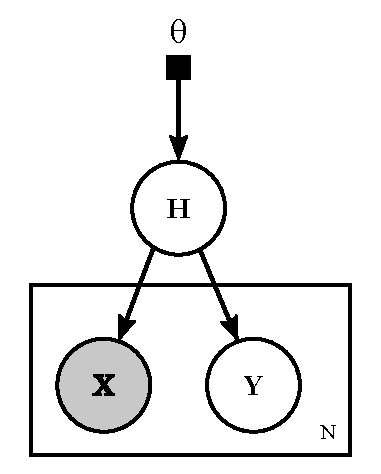
\includegraphics[width=0.33\columnwidth]{figures/probModel/probModel.pdf}}
        \caption{\label{fig:probModel} The simulator as probabilistic graphical model. The model generates $N$ pairs of images $\mathbf{X}$ and hidden joint positions in rendered images $\mathbf{Y}$. Both, $\mathbf{X}$ and $\mathbf{Y}$, are conditioned on global hidden random variables $\mathbf{H}$. Probability density functions of $\mathbf{H}$ are governed by parameters $\theta$.}
    \end{figure}

    The problem at hand is to derive the hidden joint locations $\mathbf{Y}$ in the camera images. Based on the probabilistic model alone, it is not easily possible to invert reasoning. Although we fully control the process of image generation, we have no possibility to directly infer hidden parameters $\mathbf{Y}$, given the observed images $\mathbf{X}$. 
    
    In addition to the random parameters of the simulator explained above, we use conventional data augmentation. This includes random scaling of background images, random color jitter, etc. Although this could be seen as part of the probabilistic model, it is not included in the simulator. 
    

\subsection{Localization Model and Training}
    \label{sec:model}

    Joint localization deals with the task of estimating positions of articulated body parts that constitute kinematic chains. In this work, we define joint localization as the process of predicting 2D pixel coordinates of robotic revolute joints from color image input. 
    
    Our model, outlined in Figure \ref{fig:jointmodel}, is based on the architecture proposed by Heindl et al. \cite{cheind2019disp}, which in turn is an extension to methods developed for human pose estimation \cite{cao2017realtime, newell2016stacked}. Instead of predicting sparse joint pixel coordinates, we train the network to predict dense belief maps per joint $\hat{\mathbf{B}} \in \mathbb{R}^{J \times H' \times W'}$ in the following way. Color images $\mathbf{X} \in \mathbb{R}^{3 \times H\times W}$ are input to a pre-trained VGG network \cite{simonyan2014very} to extract base features $\mathbf{F} \in \mathbb{R}^{C \times H' \times W'}$. A series of convolutional image-to-image networks refines belief predictions by allowing each network to work on the basis of outputs from the previous network and VGG base features.

    \begin{figure} [!h]
        \centering
        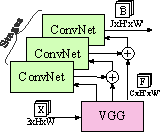
\includegraphics[width=0.7\columnwidth]{figures/joint_model/joint_model.pdf}
        \caption {
            \label{fig:jointmodel} 
            Architecture of the localization module. Each stage predicts joint belief maps. Successive stages are fed a channel concatenated stack of VGG features and the current estimate.
        }
    \end{figure}

    We generate target belief maps $\mathbf{B}$ by pixel-wise maximization over the contributions from $J$ squared exponential kernels
    \begin{equation}
        k_{\textrm{SE}}(\mathbf{p};\mathbf{y}) = \sigma^2e^{-\frac{\lVert \mathbf{p} - \mathbf{y} \rVert^2_2}{l^2}} \;\;,{\mathbf{p} \in \mathbb{R}^{H\times W}}
    \end{equation}
    centered at sparse image joint locations ${\{\mathbf{y}_0,\ldots,\mathbf{y}_J\} \subseteq \mathbb{R}^{H\times W}}$. The output variance $\sigma^2$ determines the average distance away from its mean, the length-scale $l$ determines the width of the kernel. During training, an objective function penalizes pixel-wise differences between belief predictions $\hat{\mathbf{B}}$ and targets $\mathbf{B}$ after each stage. Usually, $L_2$ or smooth $L_1$ loss functions are used. These intermediate losses help the network to train more effectively, as the effect of vanishing gradients in deep architectures is minimized \cite{newell2016stacked, wei2016convolutional}. 
    
    When predicting from the network only the output of the last stage is used. For partial scale invariance of image features, we additionally average the belief predictions of input images scaled to different resolutions.

\subsection{Feedback Mechanism}
    \label{sec:feedback}
    A key idea to our work is a feedback mechanism that enables adaptive sampling from simulator engines. As outlined in Figure \ref{fig:architecture}, a controller updates the simulation based on information of the current training mini-batch. In principle, the update can be of any kind. In this work, however, we focus on modifying probability distributions of the graphical model controlling the simulation process. In particular we modify distributions of hidden variables in such a way that more examples $\{(\textbf{x},\textbf{y},\textbf{h})\}$ of high value to the training are produced. Once a subset of important examples $\mathcal{S} = \{(\textbf{x},\textbf{y},\textbf{h})\}$ from the training batch has been selected, we infer $\mathrm{P}(\textbf{H},\textbf{Y} \lvert \textbf{X};\mathcal{S})$ (approximately, analytically or in a heuristic fashion) and continue sampling from the updated distribution.

    We propose two ways to measure the value of specific samples for training. The first utilizes the loss function to assign more importance to examples of high error. This leads to sampling strategies that put more weight into regions of high training error. The second method uses prediction uncertainty to select sample candidates. In contrast to Bayesian learning for neural networks \cite{neal2012bayesian}, deterministic regression networks do not have any meaningful measure of uncertainty built in or are not well calibrated for uncertainty estimation (in the classification case) \cite{guo2017calibration}. One way to overcome this limitation is to perform approximate Bayesian uncertainty estimation as proposed in Gal et al. \cite{gal2015dropout}. Samples selected by uncertainty are intrinsically determined by the model without consulting a loss function.
    
    %http://stillbreeze.github.io/Uncertainty-Estimation-in-Deep-Learning/

\subsection{Implementation Notes}
    \label{sec:impl}
    We use Blender 2.79 \cite{blender} as a simulator engine for robotic scenes. Blender offers great scripting support, that allows us to hook into the rendering process. Our localization model is defined and trained using PyTorch \cite{paszke2017automatic}. As communication layer we use the distributed messaging library ZeroMQ \cite{zeromq_guide}. In particular, publisher/subscriber patterns are used for broadcasting simulation results to the training loop. We limit the number of outstanding messages at the subscriber to prevent the training loop from running out of memory. The control signal is based a simple request/reply pattern. As outlined in figure \ref{fig:architecture}, TCP/IP is used as transport layer \footnote{A minimal working sample is available at \iffinalcopy \texttt{https://github.com/cheind/pytorch-blender} \else \texttt{link removed for blind review.} \fi}. We note that all relevant training data is transmitted via the communication channels without the need for temporary files.
    % TODO
    %\url{https://github.com/cheind/pytorch-blender}}.

\section{Results}

    In the following we describe the training procedure, evaluation of our method on synthetic and real world data, and provide runtime metrics.

    \subsection{Training}
    For training the localization model we sampled a set of 10.000 samples per epoch from two simulator engines. The first simulator generated uniform random poses, while the second simulator produced importance samples as described in Section \ref{sec:feedback} according to a loss metric. Two distinct collections of random background images (city and industrial theme) were used as synthetic training- and test-set backgrounds. We trained the joint localization model using six stages with input images of size $320 \times 240$. A VGG network, pre-trained on detection, was used to generate base features. We used Adam \cite{kingma2014adam}, $\eta=\num{1e-3}$, optimization with mini-batch learning for a total of 30 epochs.

    \subsection{Evaluation}
    We test the joint localization model on synthetic and real world images (see \ref{fig:posresults} for exemplary results). For comparison we extract joint locations from prediction belief maps $\hat{\mathbf{B}}$ by performing smoothed non-maximum suppression, followed by extracting the maximum peak per joint channel. For real-world images we asked a human export to annotate the joint locations. Synthetic images are auto-labelled by the simulation engine. Figure \ref{fig:posresults} provides some sample results: Robot joint locations detected by our model trained only on artificial data.
    
    We define the localization error as the Euclidean distance between predicted and target pixel locations and report it in percent of the image diagonal. Figure \ref{fig:pixelerror} shows the localization error on two distinct test sets: synthetic with random backgrounds (Figure \ref{fig:locationerror_synth}) and real-world images (Figure \ref{fig:locationerror_real}). As expected our system performs better on synthetic data than real data.
    \begin{figure}[!h]
        \centering
        \begin{subfigure}[t]{0.49\columnwidth}
            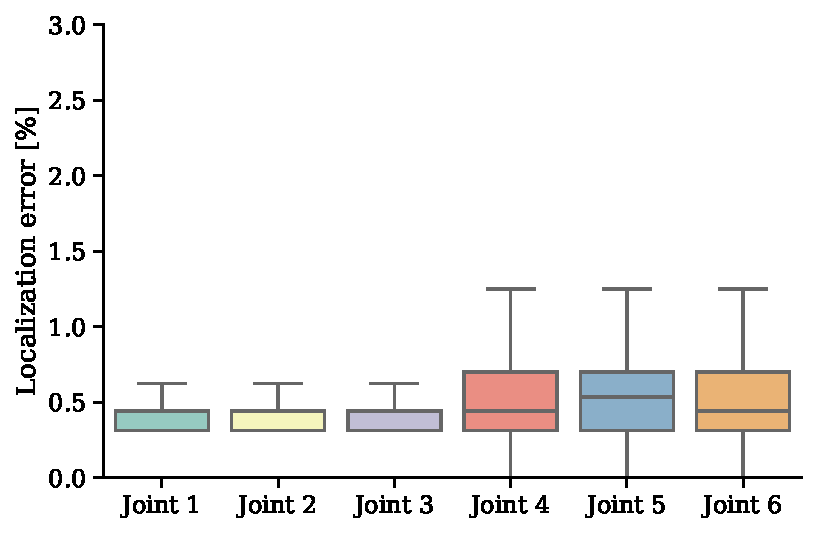
\includegraphics[width=\columnwidth]{figures/results/pixel_errors/pixel_error_synth.pdf}
            \caption {
                \label{fig:locationerror_synth} 
                Localization errors of joint prediction on a synthetic test data set with auto-labelled ground truth.
            }
        \end{subfigure}
        \begin{subfigure}[t]{0.49\columnwidth}
            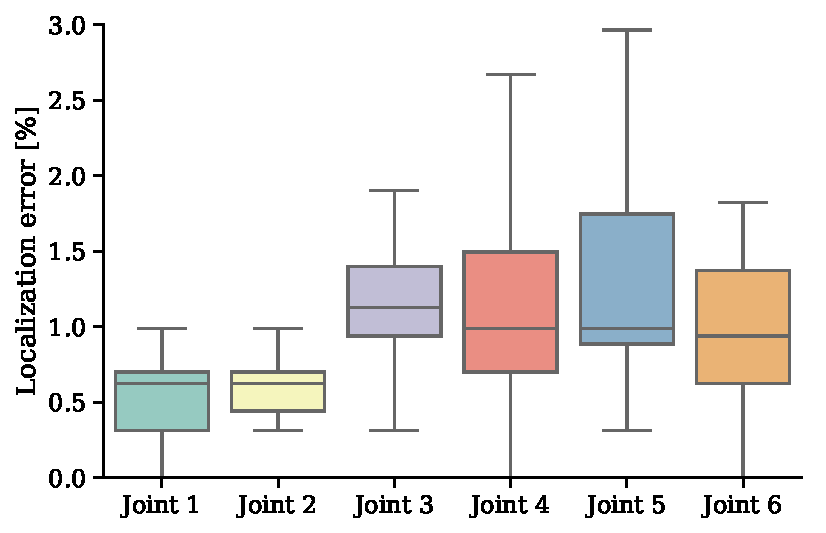
\includegraphics[width=\columnwidth]{figures/results/pixel_errors/pixel_error_real.pdf}
            \caption {
                \label{fig:locationerror_real} 
                Localization errors of joint prediction for a real world test set. Target locations annotated by a human domain expert. 
            }
        \end{subfigure}
        \caption {
            \label{fig:pixelerror} 
            Localization errors of robot joint prediction. Results are in percent of image diagonal.
        }
    \end{figure}
    We attribute two effects for this outcome: (a) our simulation is non-realistic and (b) human annotation is error-prone. To underpin the latter claim, we have conducted a pilot study in which 10 people (all with reference to robotics) annotated 12 real world images of an UR-10 robot in different poses and from different viewpoints. We then computed the inter-rater spread as measure of confidence for human annotations in our domain. Figure \ref{fig:humanuncertainty} shows the average uncertainty per joint over all images. We find that the middle joints, often blocked by view and robot pose, are the most difficult to annotate precisely. These results indicate that our method (figure \ref{fig:locationerror_real} right) performs quite well.

    \begin{figure}[!h]
        \centering
        \begin{subfigure}[t]{0.49\columnwidth}
            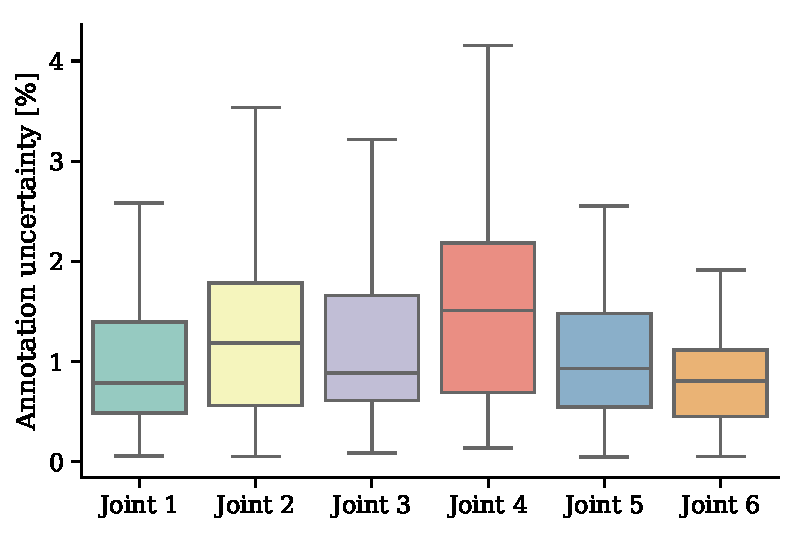
\includegraphics[width=\columnwidth]{figures/results/human_uncertainty/human_uncertainty.pdf}
            \caption {
                \label{fig:humanuncertainty} 
                Human uncertainty estimates in pose annotation. Results are in percent of image diagonal.
            }
        \end{subfigure}
        \begin{subfigure}[t]{0.49\columnwidth}
            \iffinalcopy
                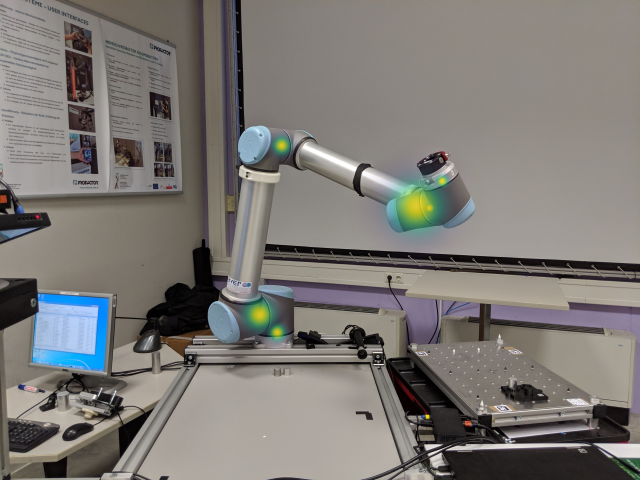
\includegraphics[width=\columnwidth]{figures/results/human_uncertainty/human_uncertainty_belief.png}
            \else
                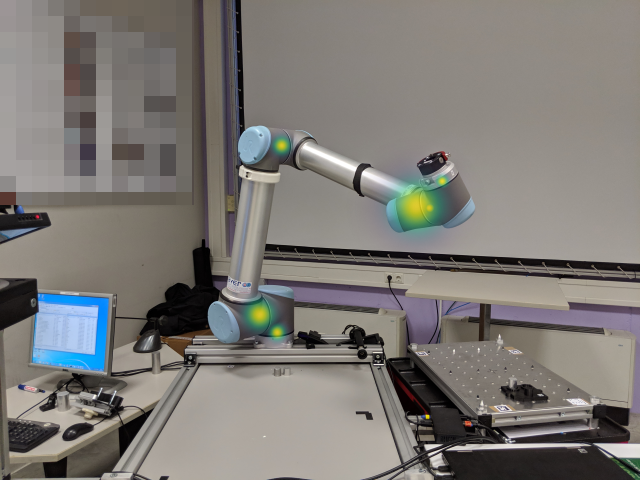
\includegraphics[width=\columnwidth]{figures/results/human_uncertainty/human_uncertainty_belief_blind.png}
            \fi
            \caption {
                \label{fig:humanuncertainty_belief} 
                Uncertainty estimates superimposed as Gaussian kernels on one of the images to be annotated.
                \iffinalcopy
                \else
                    \texttt{Image backgrounds modified for blind review.}
                \fi
            }
        \end{subfigure}
        \caption {
            \label{fig:uncertainty} 
            Uncertainty estimates from human annotation. Results are in percent of image diagonal.
        }
    \end{figure}

    \begin{figure}[htbp]
        \centerline{
            \iffinalcopy
                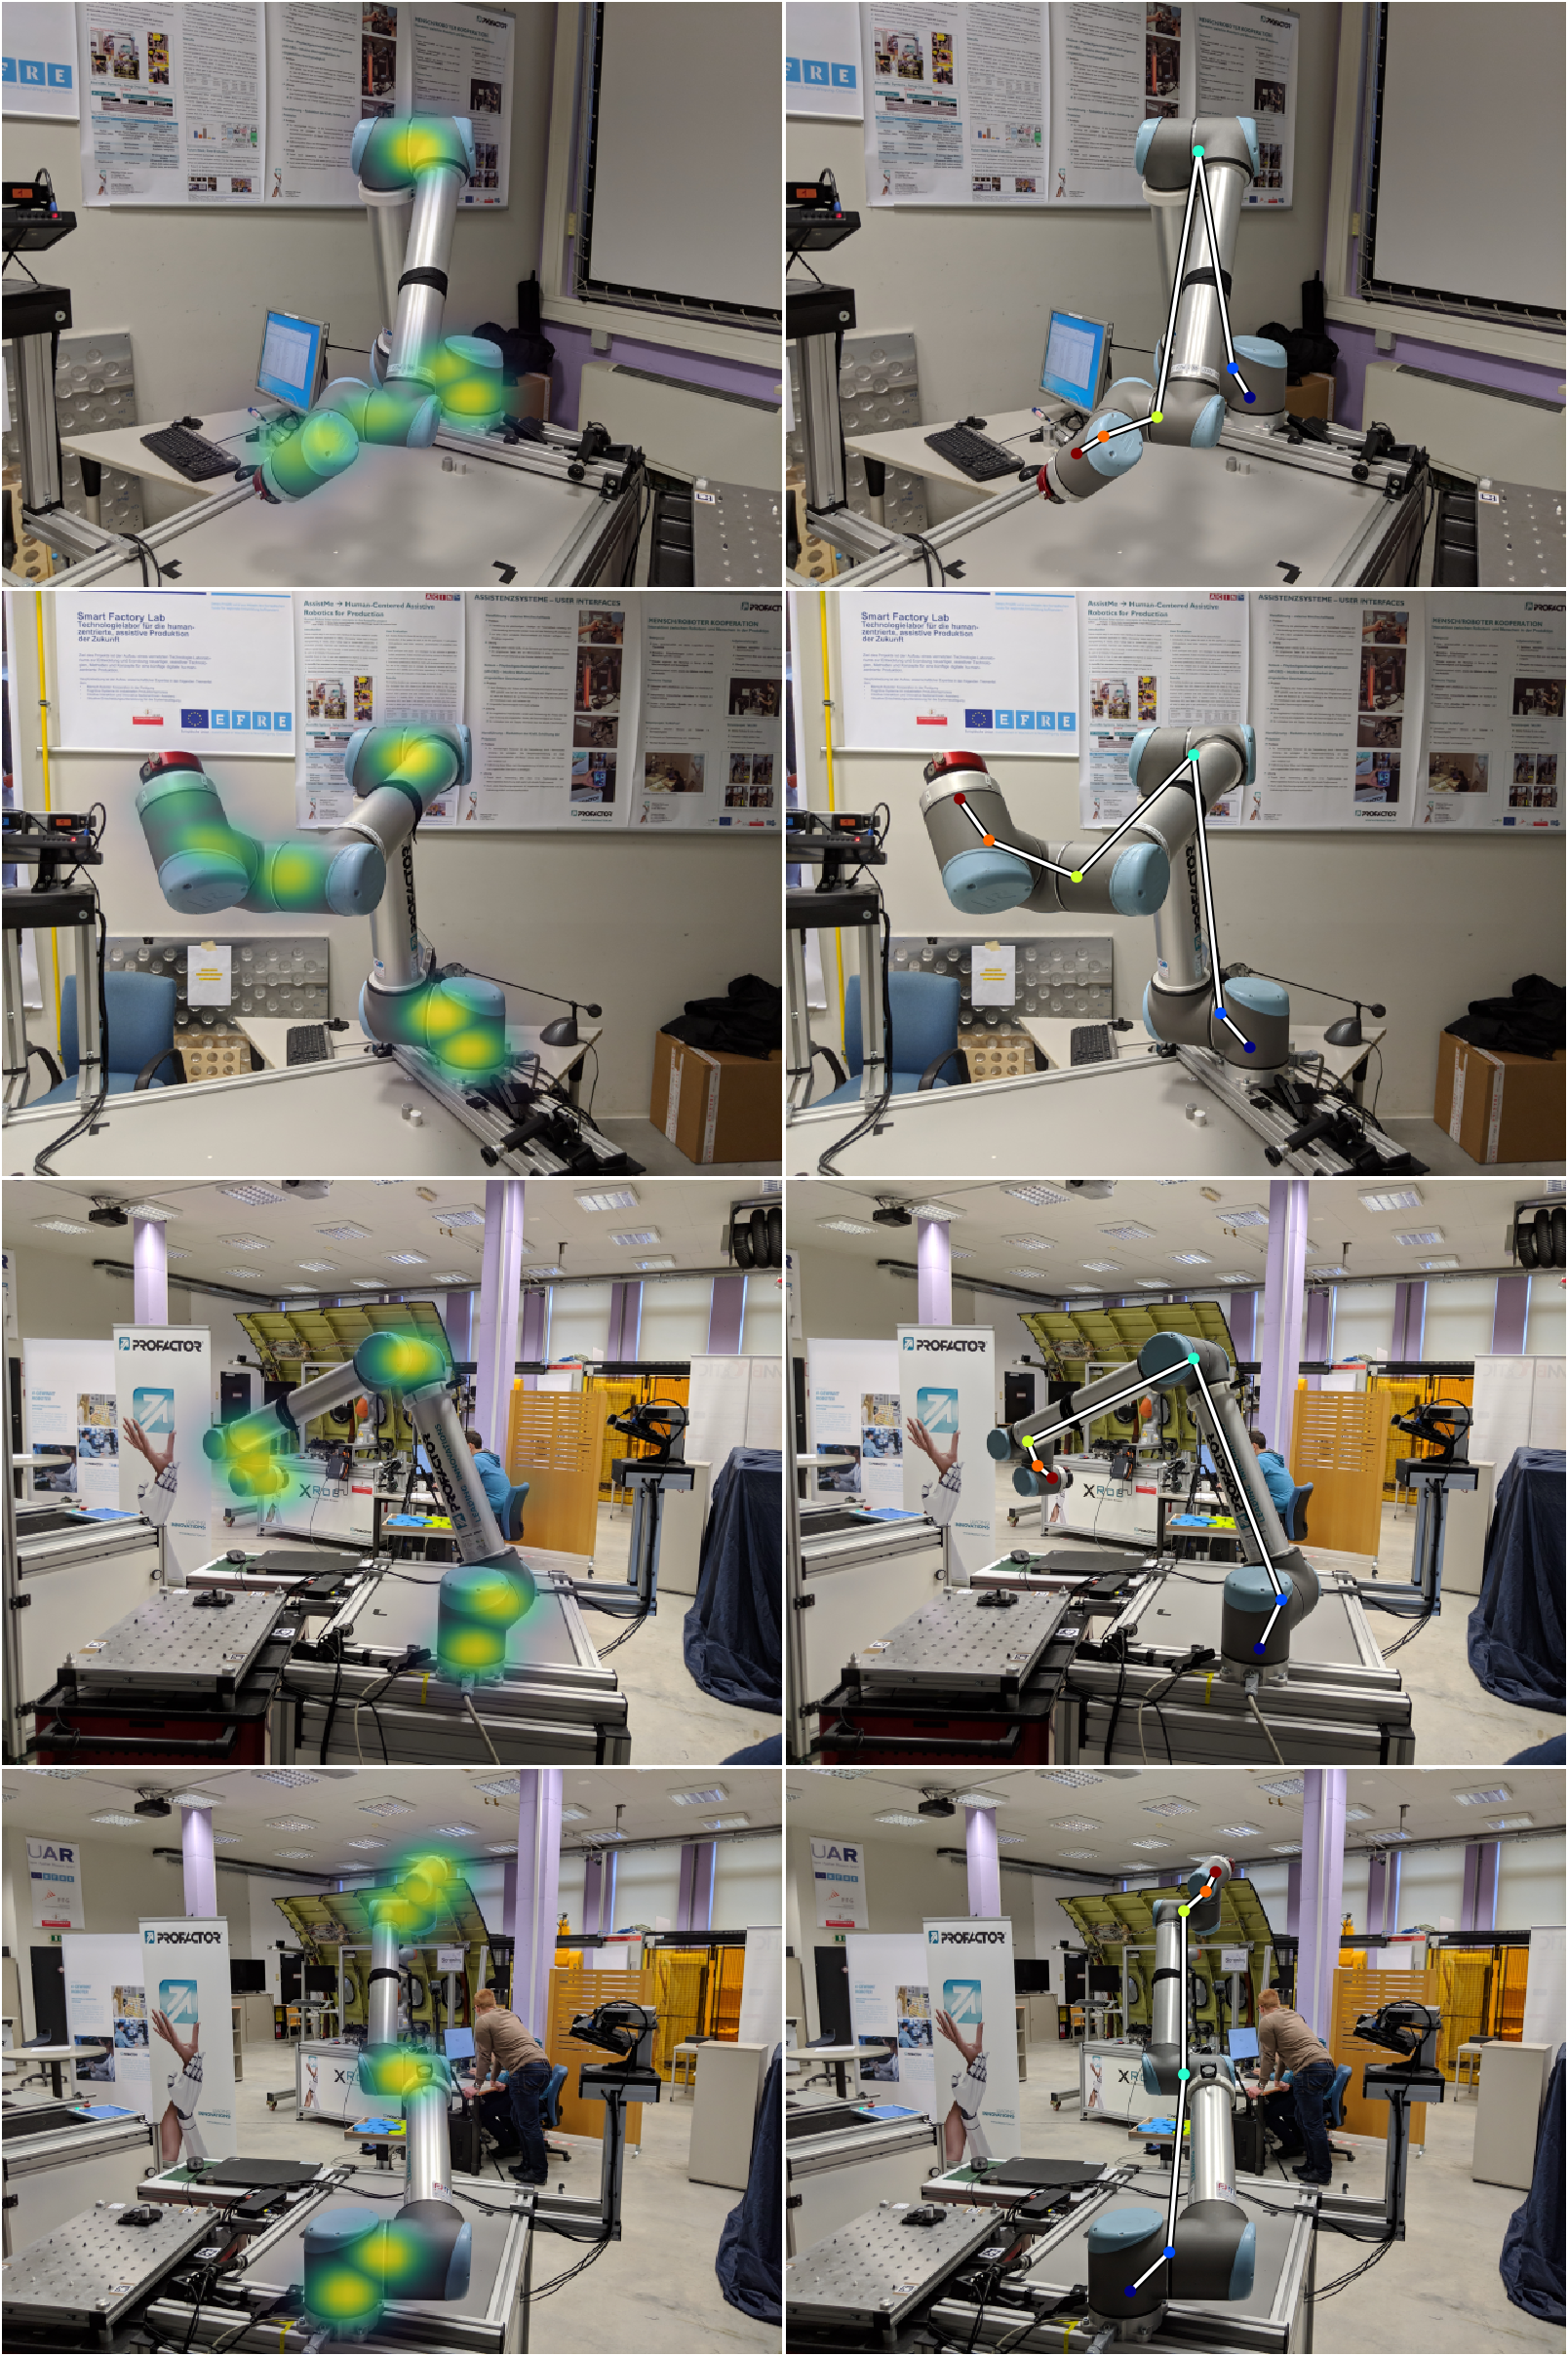
\includegraphics[width=0.98\columnwidth]{figures/results/ur10_lab/mosaic.png}
            \else
                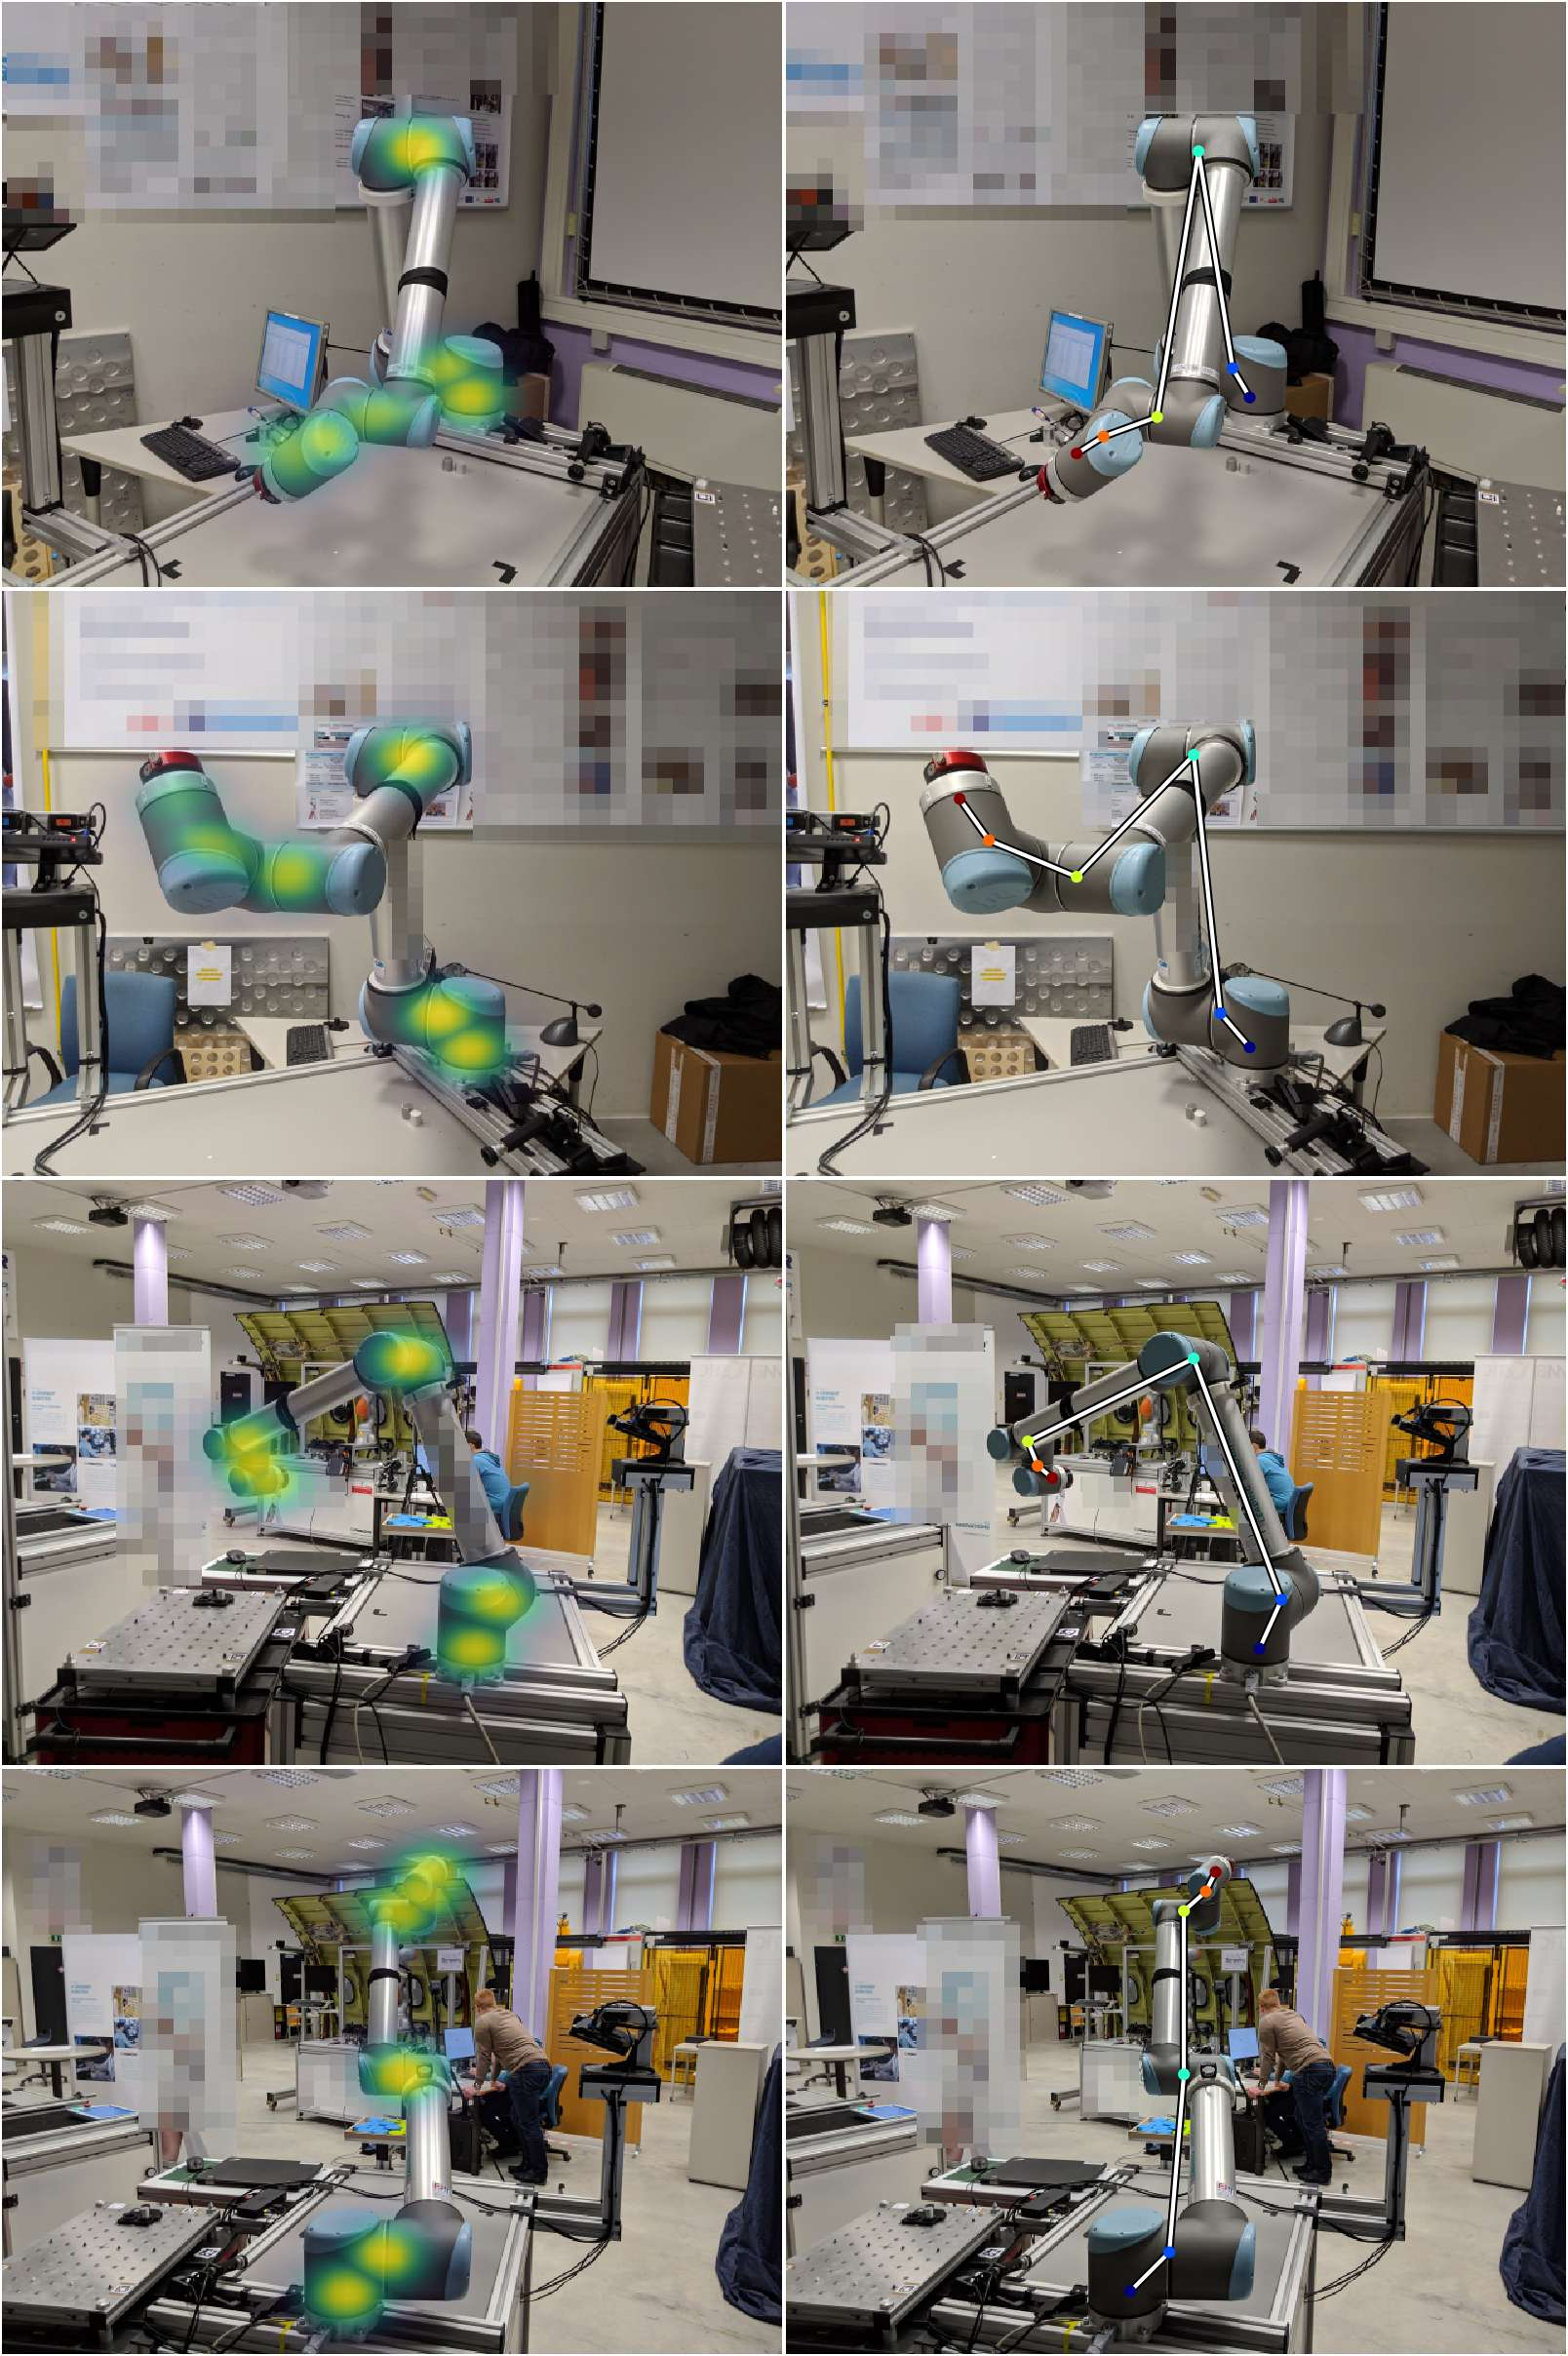
\includegraphics[width=0.98\columnwidth]{figures/results/ur10_lab/mosaic_blind.jpg}
            \fi
            }
        \caption{
            \label{fig:posresults} Samples from our real-world database. Predicted belief maps (left-column) and extracted joint coordinates (right-column) dataset. 
            \iffinalcopy
            \else
                \texttt{Image backgrounds modified for blind review.}
            \fi
        }
    \end{figure}

    \subsection{Effects of Feedback}
    We evaluate the effectiveness of our feedback mechanism to generate adapted samples in the following way: a training is run twice, once without feedback enabled and one time with adaptive feedback for 30 epochs each. Each run spawns two simulator engines. In the feedback enabled run, a high $L_2$ loss indicates examples that should be resampled. We then adapt the prior distributions over joint angles of the second simulator to generate more samples in close vicinity of important joint angle configurations. To avoid too heavy exploitation behavior in training, the generated samples are interleaved at the subscriber. This ensure half of the training examples come from each of the simulators. Figure \ref{fig:control} shows the beneficial effects of our approach. Note, we only change the distribution of joint angles and leave all distributions unchanged. As described in Section \ref{sec:feedback}, one should ideally update $\mathrm{P}(\textbf{H},\textbf{Y} \lvert \textbf{X};\mathcal{S})$ for all hidden variables.

    \begin{figure}[htbp]
        \centerline{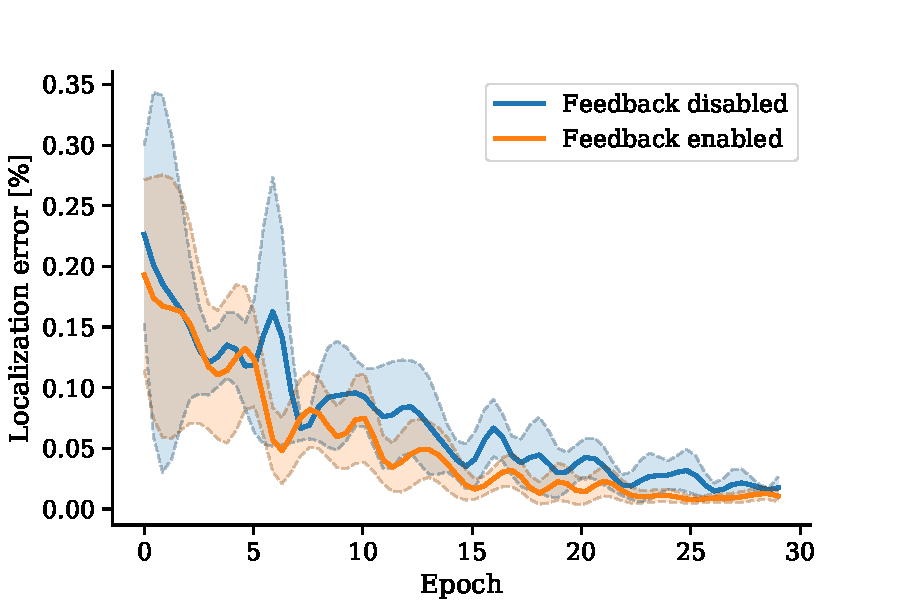
\includegraphics[width=0.9\columnwidth]{figures/control/control.pdf}}
        \caption{
            \label{fig:control} Effects of applying adaptive simulator feedback comparing two trainings over 30 epochs. We see faster convergence if we let one of the simulator instances generate more examples in the neighborhood of training samples with high errors. Errors are in percent of image diagonal.
        }
    \end{figure}

    \subsection{Runtime Analysis}
    All experiments are performed on a computer with 2x Intel Xeon E5-2650v4 12-Core and 4 NVIDIA Tesla V100 SXM2 32 GB GPUs. Table \ref{tab:runtime} summarizes the individual runtimes of different parts of our system. Through parallelization, our framework is capable of producing samples fast enough to avoid stalling network training.

    \begin{table}
        \centering
        \begin{tabular}{lrr}
            \toprule
            {} &  Mean [ms] &  Std [ms] \\
            Task                   &            &           \\
            \midrule
            Simulation step        &      250.32 &    10.21  \\
            Batch collating (8/8)  &      321.23 &    24.76  \\
            Train step             &      521.23 &   73.76  \\
            Prediction             &      95.21 &    14.32 \\
            \bottomrule
        \end{tabular}
        \caption{
            \label{tab:runtime} 
            Runtimes of different parts of our pipeline for $320 \times 240$ input images. All timings in milliseconds. Simulation step refers to the generation of a single training sample. Batch collating (8/8) means waiting for a batch-size of eight samples from eight simulator instances. Train step includes timings of forward and backward network passes. Prediction refers to the duration of predicting belief maps for a single input image.
        }
    \end{table}

\section{Discussion}
This work considers a new approach to train from artificial images in the area of robot pose estimation. We show that a non photo-realistic simulation suffices to learn models that are capable of detecting robots in real world images. Additionally, our architecture enables the training procedure to directly communicate with the simulator. This leads to more effective training as samples can be generated on the fly based on the requirements of model learning.

In the future we would like to investigate additional methods to constrain robot poses in images. The prediction of joint angles would help to reconstruct 3D poses of robots in 2D color images. One of the drawbacks of the current method is that it only reliably works for a single robot in the scene. While multi-pose detectors for robots have been considered in the past \cite{cheind2019disp}, these methods are not independent of the number robots in the scene (with respect to runtime complexity). We therefore see the need for more research in this direction, paving the way to real-time pose detection in the wild.

\section*{Acknowledgment}
\iffinalcopy
This research was supported in part by ”FTI Struktur Land Oberoesterreich (2017-2020)”, the European Union in cooperation with the State of Upper Austria within the project Investition in Wachstum und Beschäftigung (IWB).
\else
\texttt{Acknowledgment removed for blind review.}
\fi

\small
\bibliographystyle{ieeetr}
\bibliography{biblio}

\end{document}
